Cooling the two KID arrays at about 100~mK is the major requirement for
driving the architecture of the \NIKA\ instrument. This is achieved by a 4~K
cryocooler and a closed-cycle $^3$He - $^4$He dilution.  The optical coupling
between the telescope and the detectors is made by warm aluminum mirrors and
cold refractive optics.  The optics consists of a flat mirror at the
top of the cryostat, an off-axis biconic-polynomial curved mirror, a 300~K
window lens, a field stop, a 4~K lens, an aperture stop, a dichroic, a 100~mK
lens, and two band-defining filters in front of the back-illuminated KID
arrays, which have a backshort that matches the corresponding wavelength.  A view
of the optics of the \NIKA\ instrument and the coupling with the 30~m
telescope is presented in Fig. \ref{fig:optics}.  All the elements presented
in this figure are real optical elements except for the vertical segment
showing the entrance of the receiver cabin and the vertical segments inside
the cryostat (field and pupil diaphragms, filters, dichroic and detector
arrays). 

The throughput of each pixel is calculated using the knowledge of the telescope diameter and equivalent focus, the fraction of unvignetted pupil defined by the cold field stop, and the receiver pixel (KID) size with respect to diffraction pattern. Using $A$ for Area, $\Omega$ for solid angle, $u$ for pixel size in unit of $F \lambda$ ($\lambda$ = wavelength and F= f-number or relative aperture), we have
$$
A\Omega_{pixel} = \frac{A_{M1} (u F \lambda)^2}{f^2_{eq}} = (\pi/4)  (u \lambda)^2 .
$$
where $A_{M1}$ is the effective primary mirror diameter, and $f_{eq}$ the equivalent focal of the telescope.
The effective throughput of the instrument is then $A \Omega_{effective} = N*A\Omega_{pixel}$, where N is the number of valid receiver pixels. 


\begin{figure}[t!]
\begin{center}
\includegraphics[scale=0.25]{figures/optics_11.eps}
\includegraphics[scale=0.25]{figures/optics_2.eps}
\end{center}
\caption{Snapshot from the Zemax simulation used to optimize the optical
  system of \NIKA. In the order of photon travel, the \NIKA\ optics consist of a flat mirror at the top of the cryostat, an off-axis biconic-polynomial curved mirror, a 300 K window lens, a field stop, a 4 K lens, an aperture stop, a dichroic, a 100 mK lens, and two band- defining filters in front of the back-illuminated KID arrays. Top panel: ray tracing from the entrance of the
  receiver cabin of the 30~m telescope (which is simulated but not shown in the
  image), view from the elevation axis (which is symbolized by the big circles
  and contains the 2 mirrors of the Nasmyth system). The \NIKA\ cryostat and
  entrance nose are represented by the rectangles. Bottom panel: zoomed plot of the optical system inside the \NIKA\ cryostat. The angular size, the beam efficiency and the overall optical efficiency of the system are presented in Table~\ref{tab:nika_char}.}
\label{fig:optics}
   \end{figure}

   The rejection of out-of-band emission from the sky and the telescope is achieved
   by using a series of low-pass metal mesh filters, placed at different
   cryogenic stages in order to minimize the thermal loading on the
   detectors. This determines the shape, width, and position of each of the \NIKA\
   bands.  Spectral characterization of the \NIKA\ bandpass was performed using a
   Martin-Puplett interferometer allowing recovery of the spectral performance
   of each pixel of the two \NIKA\ channels with uncertenties of a few
   percent. In Fig \ref{fig:bandpass} we present the \NIKA\ bandpasses, together
   with the ATM model calculated for different water vapor contents
   (\cite{2001IEEE....49.1683C}). According to the Pardo model, the 1.25~mm
   channel is almost sensitive exclusively to the water vapor emission (water vapor
   secondary line at 183~GHz) in contrast to the 2.14~mm channel, which is slightly sensitive to the roto-vibrational emission line of dioxygen (at 119~GHz). ATM also predicts the 
   contributions of minor species like ozone to the atmospheric absorption. These
   additional contributions are ignored in this paper. Changing the
   precipitable water vapor (pwv) content in the ATM model, we can derive the
   expected sky opacities integrated into the \NIKA\ channels. The ratio between the
   opacities derived for the 1.25~mm and 2.14~mm channels is obtained not only
   according to the pseudo continuum emission of the atmosphere (proportional
   to $\nu^2$ where $\nu$ represents the electromagnetic frequency) but also taking the contribution of the water vapor emission and dioxygen emission into account.  Furthermore, between the 2012 and 2013
   observing campaigns we changed (for technical reasons) the cold optical filter 
   chain by adding a low pass filter with a
   cut-off at 270GHz. Therefore, we expect to have a different ratio in the
   derived sky opacities at 1.25~mm and 2.14~mm channels between the two campaigns. From
   the model, we obtain a ratio between the in-band sky opacities $\tau(2.14~mm)/\tau(1.25~mm)$ of 0.75 and 0.6 for the 2012 and 2013 observing campaigns, respectively.

\begin{figure}[t]
\begin{center}
\includegraphics[scale=0.52]{figures/pass_band_ATM.ps}
\end{center}
\caption{\NIKA\ bandpasses.  The bandpass of the 1.25~mm channel (resp. 2.14~mm)
  is shown in red (resp. blue). The bandpasses are averaged over all valid
  pixels, with dispersion (rms) of 2~\% at 1.25~mm and 1~\% at 2.14~mm.  The ATM
  model calculated for different water vapor contents is presented in green.}
\label{fig:bandpass}
   \end{figure}


\begin{table*}
\begin{center}
\begin{tabular}{ccc}
\hline
\hline
 & 1.25~mm channel &  2.14~mm channel  \\
\hline \hline
Pixel size [mm] & 1.6   & 2.3 \\
Dual polarization &  yes & yes \\
Angular size ($F \lambda$) &  0.9 & 0.79 \\
Beam efficiency [\%] &  55 & 70 \\
Detector efficiency [\%] & 80 & 80 \\
Overall optical efficiency [\%] &  30 & 30  \\
Total background [pW] &  45 & 20  \\
\hline \hline
\end{tabular}
\end{center}
\caption{Characteristics of the NIKA instrument coupled to the IRAM telescope. The total background is calculated per pixel with a contribution of the atmosphere derived in good weather conditions. This corresponds to an expected photon-noise level equal to about $5 \cdot 10^{-17} W/\sqrt{Hz}$ for the 2.14mm channel and $9 \cdot 10^{-17} W/\sqrt{Hz}$ for the 1.25mm channel. These parameters have a 50\% precision level.}
\label{tab:nika_char}
\end{table*}

%

\subsection{Detector array configurations}\label{dac}
%KID
The \NIKA\ LEKID detector arrays are made of aluminum and are sensitive to dual polarization. The need to have a symmetric design with a constant filling factor over the whole direct sensitive area drives us to use Hilbert fractal design, which is a well-known geometry for patch antennas (\cite{Roesch2012}). The gap of the Al films has been measured thanks to absorption spectra taken in the lab using a Martin-Pupplet interferometer. The measurements show that below roughly 110~GHz, no radiation is absorbed, meaning that the energy gap in the case of 18nm Al films is approximately 0.2~meV, and the Tc around 1.45~K. The expected film impedance (with respect to the incoming photon able to break Cooper pairs) is actually that of the normal film state. This has been measured to be around 2~$\Omega$/square. This value has been used when designing the detectors to match their effective impedance to that of the incoming radiation (which is absorbed from the substrate side, in a \textit{back-illumination} configuration).

The results reported in this paper cover two different observing campaigns at the telescope, with slightly different properties of the two focal planes:


\begin{figure}[t!]
\begin{center}
\begin{tabular}{c}
\hspace{0.5cm}
\includegraphics[bb = 1 1 170 104,width=6.4cm,clip]{figures/bonding_articoloNIKA3.eps}\\
\includegraphics[bb = 2 238 562 598,width=7cm,clip]{figures/sweep_beforeAndAfterBondings.eps}
\end{tabular}
\end{center}
\caption{Image of the bondings added across the feedline (top). As can be seen
  in the frequency sweep carried out before  (blue) and after (red) adding the bondings
  (bottom), the depth of the different resonances has become much more
  uniform, since the coupling of the resonators to the feedline is no longer
  affected by the presence of standing waves supported by the slotline
  modes. Such standing waves were also responsible of the larger dips that are
  observed before adding the bondings, and they disappear afterwards.}
\label{fig:bondings}
\end{figure}

\begin{itemize}
\item{\textbf{Campaign 11/2012}. During this campaign, referred to as Run 5,
    the 2.14~mm array is made of 132 pixels with a 20~nm thick Al film on a
    300~$\mu$m HR silicon substrate. The 1.25~mm array consists of 224~pixels
    with a film of the same thickness but on a 180~$\mu$m substrate. The cold
    amplifier of the 240~GHz channel showed an unexpectedly low saturation
    power, so that we could simultaneously read only eight pixels out with the
    ideal excitation level or, alternatively, 90 pixels but with a lower power
    per tone, resulting in suboptimal performance.  The number of valid
    pixels were 100 and 80 for the 2.14~mm and 1.25~mm channels, respectively.
    The configuration adopted during this observing campaign limited the final sensitivity of the instrument. 
    The channel at 2.14~mm (changed for the 2013 campaign) was limited by the detector noise. For the 1.25~mm channel, 
    the detectors noise was always relatively flat. This means that the intrinsic frequency noise 
    due to random variations of the effective dielectric is negligible compared to the sky noise. 
    The cold amplifier temperature noise was also negligible compared to the sky noise.}
\item{\textbf{Campaign 06/2013}. This campaign is referred to as Run 6. For
    the 2.14~mm channel, we replaced the array with a new one, obtained from a
    thinner Al film (18~nm), in which we optimized the coupling further to the
    feedline. We also added bondings across the feedline to suppress spurious
    slotline modes that were affecting the uniformity of the pixel properties,
    which led to an increase in the number of valid pixels (figure
    \ref{fig:bondings}). The overall geometry and the pitch between pixels
    was left unchanged, as was the readout chain. For the 1.25~mm channel, the
    only intervention was to replace the cold amplifier with a new one
    having a higher power handling. RF filters have also been added on the
    readout chain to avoid the harmonics of the local oscillator from
    reaching the cold amplifier input. Since we suspected that the optical
    load on the 1.25~mm array was preventing it from cooling down
    appropriately, we added an additional low-pass edge filter cutting
    frequencies above 270~GHz, even though this led to the loss of a fraction %  (roughly $XX\%$) 
    of the power available in the atmospheric window of
    interest. The number of valid pixels for this campaign was 125 at 2.14~mm
    and 190 at 1.25~mm, for a total of 315 pixels.
   This new configuration was expected to yield a much improved low noise performance, but the bad weather 
   during the observing campaign limited the sensitivity of our arrays. For both channels the dominant noise contribution was due to residual sky noise associated to atmospheric turbulences and residual correlated electronic noise.}
\end{itemize}



%\textcolor{blue}{MC: it is well NIKEL v1 (at least in 'our' dictionary..). In any case, what about leaving out the details that were here (and that furthermore were not accurate at all)? I'd go for something more 'qualitative' like:}

%During the observing campaign 2012 the channel at 2.14mm was limited by the detector noise. Except for this array (that we changed for the 2013 campaign) the detectors noise was always relatively flat. This means that the intrinsic frequency noise due to random variations of the effective dielectric is negligible compared to the sky noise. Finally the cold amplifier temperature noise is also negligible compared to the sky noise.

For the readout, we used the new NIKEL version 1 electronics, which have
worked flawlessly. The boards, described in detail in \cite{Bourrion2012}, are
capable of generating up to 400 tones each over a 500~MHz bandwidth. This is
achieved by using six separate FPGAs: five of them generate 80 tones each over a
100~MHz band, using five associated DACs. The sixth FPGA acts as a central unit
that combines the signal of the other units, apprioprately shifting and
filtering the different 100~MHz sub-bands to finally cover the whole 500~MHz
available for the frequency comb used to excite the detectors. An analogous,
but reversed, process is then applied to the signal acquired by the ADC of the
board, which is once again split in five different sub-bands treated
separately. Each NIKEL v1 board thus allows us to monitor all the 400 tones
simultaneously with a margin of two bits in the 12 bits ADC dynamics.

%After propagating through the cryostat, this signal arrives at the input of the ADC of the board then undergoes an analogous, but reversed, process in order to separate the 5 sub-bands.

%REU    TO  BE  IMPROVED!


Data are acquired at a 23.842~Hz rate, synchronously over the two arrays. Binary
files are provided as output, which contain the raw data, as well as the
resonant frequency of each KID used to set the corresponding excitation tone.

The principal characteristics of the NIKA instrument are presented in Table \ref{tab:nika_char}. 

%The table has to be considered as a good indication of the characteristic of the NIKA instrument.


